\documentclass[letterpaper,11pt,notitlepage,fleqn]{article}

%\usepackage{nopageno} %gets rid of page numbers
\usepackage{alltt}                                           
\usepackage{float}
\usepackage{color}
\usepackage{indentfirst}
\usepackage{url}
\usepackage{balance}
\usepackage[TABBOTCAP, tight]{subfigure}
\usepackage{enumitem}
\usepackage{pstricks, pst-node}
\usepackage{geometry}
\geometry{textheight=9in, textwidth=6.5in} %sets 1" margins 
\newcommand{\cred}[1]{{\color{red}#1}} %command to change font to red
\newcommand{\cblue}[1]{{\color{blue}#1}} % ...blue
\usepackage{hyperref}
\usepackage{textcomp}
\usepackage{listings}
\usepackage{graphicx}
\usepackage{amsfonts}
\usepackage{amsmath}

% Code snippets color
\definecolor{dkgreen}{rgb}{0,0.6,0}
\definecolor{gray}{rgb}{0.5,0.5,0.5}
\definecolor{mauve}{rgb}{0.58,0,0.82}
\lstset{frame=tb,
  language=C,
  aboveskip=3mm,
  belowskip=3mm,
  showstringspaces=false,
  columns=flexible,
  basicstyle={\small\ttfamily},
  numbers=none,
  numberstyle=\tiny\color{gray},
  keywordstyle=\color{blue},
  commentstyle=\color{dkgreen},
  stringstyle=\color{mauve},
  breaklines=true,
  breakatwhitespace=true,
  tabsize=3
}
\lstdefinelanguage{diff}{
    morecomment=[f][\color{blue}]{@@},     % group identifier
  morecomment=[f][\color{red}]-,         % deleted lines 
  morecomment=[f][\color{green}]+,       % added lines
  morecomment=[f][\color{magenta}]{---}, % Diff header lines (must appear after +,-)
  morecomment=[f][\color{magenta}]{+++},
}
% End color
\def\name{Sam Quinn}

\parindent = 0.4444 in
\parskip = 0.2 in

\begin{document}
\begin{titlepage}
    \vspace*{\fill}

    \newcommand{\HRule}{\rule{\linewidth}{0.5mm}} % Defines a new command for the horizontal lines, change thickness here

    \center % Center everything on the page

    %----------------------------------------------------------------------------------------
    %TITLE SECTION
    %----------------------------------------------------------------------------------------

    %\includegraphics[scale=.5]{image.eps}
    \HRule \\[0.4cm]
    { \huge \bfseries Homework \#1}\\[0.4cm] % Title of your document

    %----------------------------------------------------------------------------------------
    %HEADING SECTIONS
    %----------------------------------------------------------------------------------------

    \textsc{\LARGE Oregon State University}\\[0.5cm] % Name of your university/college
    \textsc{\Large ECE 478 Network Security}\\[0.5cm] % Major heading such as course name
    \textsc{\large Spring 2016}\\[0.5cm] % Minor heading such as course title


    \HRule \\[1.5cm]
    %----------------------------------------------------------------------------------------
    %AUTHOR SECTION
    %------------------------------------ ----------------------------------------------------

    \begin{minipage}{0.4\textwidth}
        \begin{flushleft} \large
            \emph{Student:}\\
            \noindent \textbf{Sam \textsc{Quinn}} \\ % Your name
            {\small Quinnsa@Oregonstate.edu}
        \end{flushleft}
    \end{minipage}
        ~
        \begin{minipage}{0.4\textwidth}
            \begin{flushright} \large
                \emph{Professor:} \\
                \noindent \textbf{Dr. Attila A \textsc{Yavuz}} \\ % Supervisor's Name
                {\small Attila.Yavuz@oregonstate.edu}
            \end{flushright}
        \end{minipage}\\[3cm]

        %----------------------------------------------------------------------------------------
        %DATE SECTION
        %-----------------    -----------------------------------------------------------------------

    {\large \today}\\[3cm] % Date, change the \today to a set date if you want to be precise

    %----------------------------------------------------------------------------------------
    %LOGO SECTION
    %------   ----------------------------------------------------------------------------------

    
\includegraphics[scale=0.5]{coe.eps}\\[1cm] % Include a department/university logo - this will require the graphicx package

    %----------------------------------------------------------------------------------------

    \vfill % Fill the rest of the page with whitespace



\end{titlepage}

\tableofcontents
\newpage
\section{[24] Merkle Hash Tree}
%\Tree[.1$\Box\Box\Box\Box$ [.2$\Box\Box\Box\Box$ [.4$\Box\Box\Box\Box$ $\Box\Box{b1}\Box$\\8 $\Box\Box\Box{b2}$\\9 ][.5$\Box\Box\Box\Box$ $\Box\Box\Box{b3}$\\10 $\Box{b4}\Box\Box$\\11 ]][.3$\Box\Box\Box\Box$ [.6$\Box\Box\Box\Box$ ${b5}\Box\Box\Box$\\12 $\Box\Box{b6}\Box$\\13 ][.7$\Box\Box\Box\Box$ $\Box{b7}\Box\Box$\\14 ${b8}\Box\Box\Box$\\15 ]]]
\begin{center}
    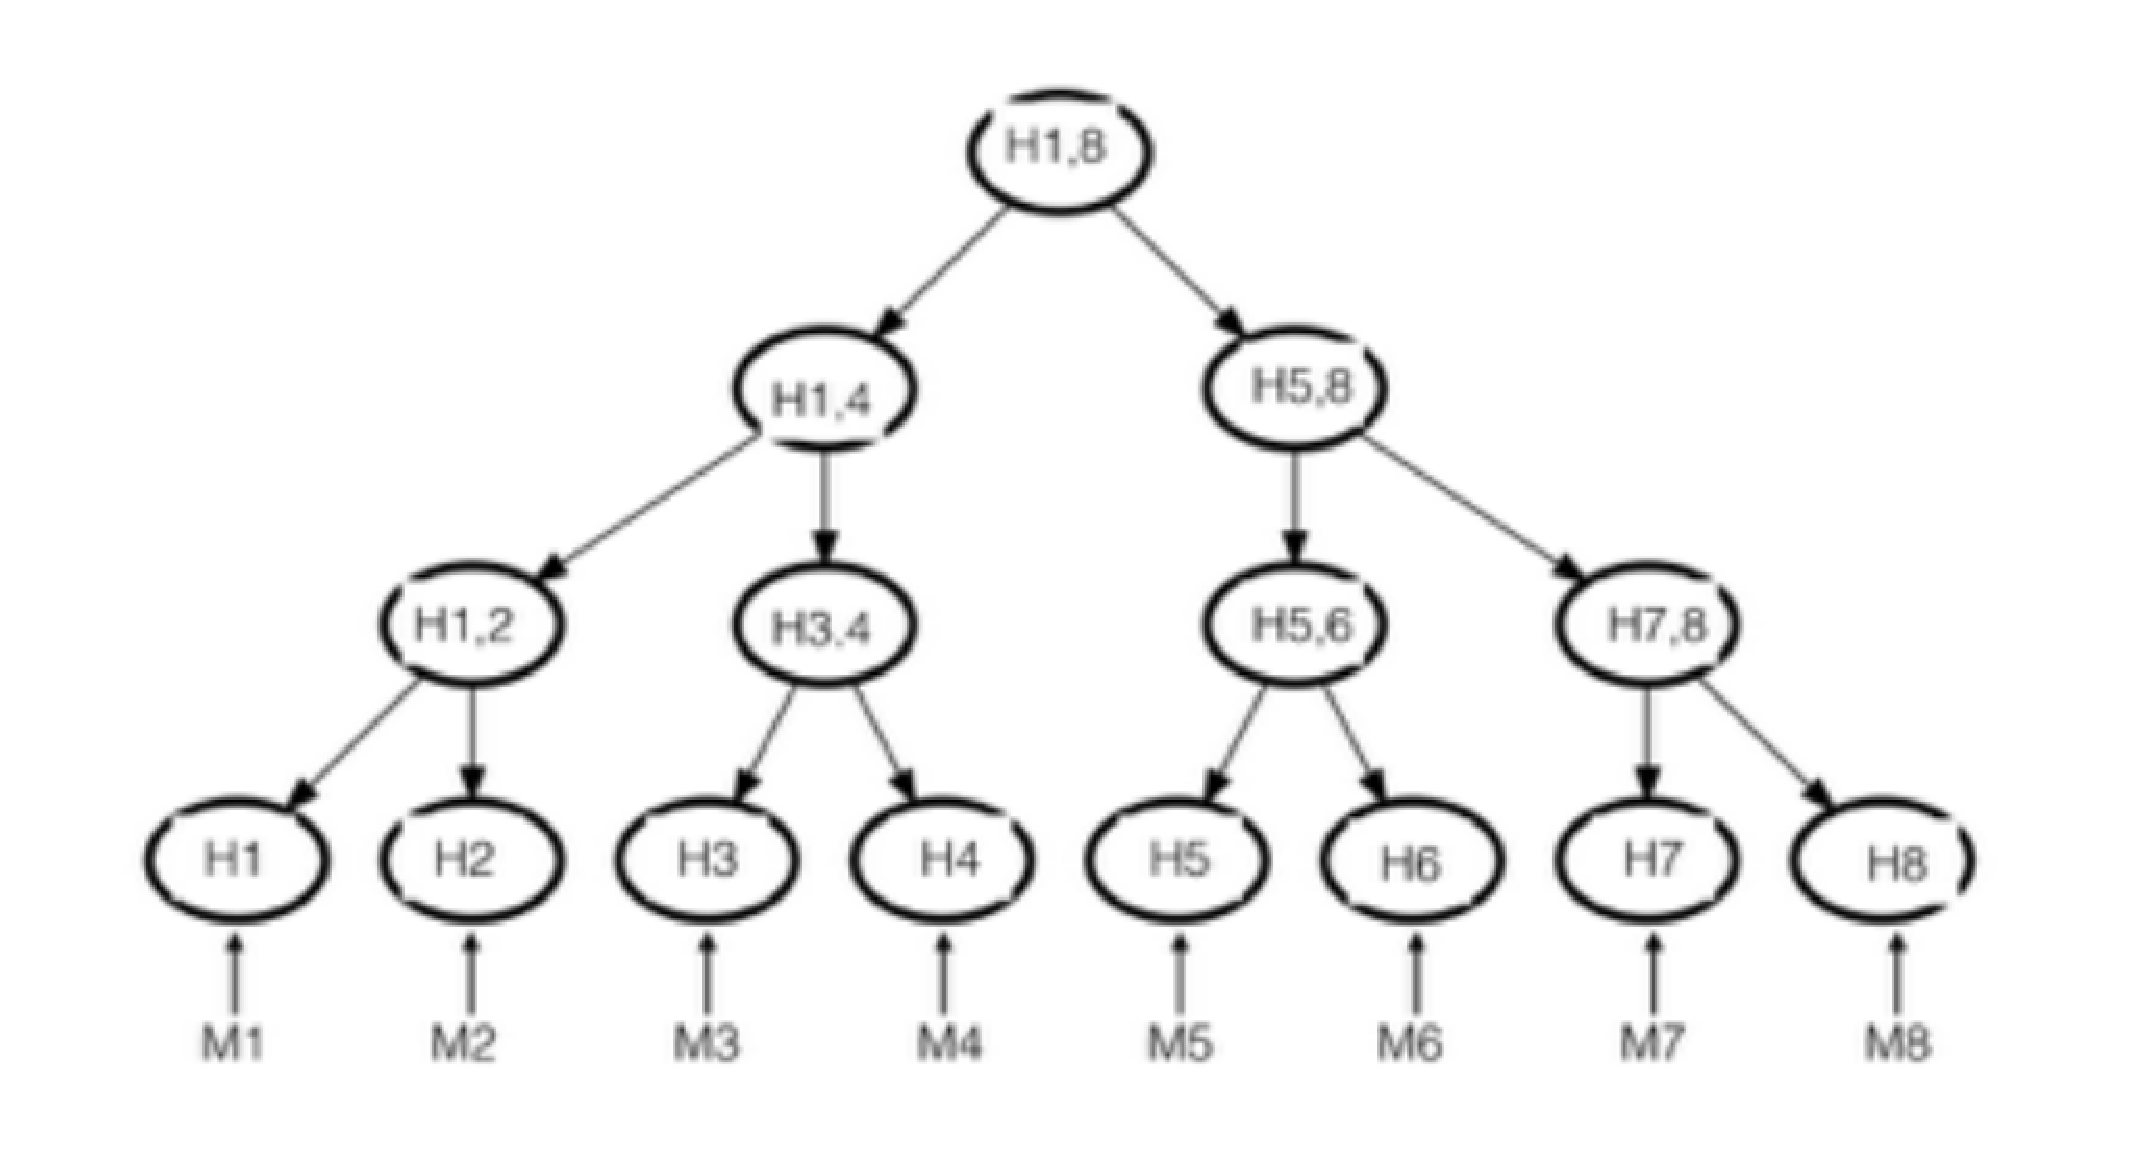
\includegraphics[scale=0.5]{tree.eps}
\end{center}

\noindent \textbf{Suppose a sender S uses this Merkle hash tree to authenticate these messages to a receiver R. What should be done before this tree can be used?}

Before the Merkle hash tree is able to be sent the root of the tree (H1,8) must be authenticated. This is tyically done through a digital signatuer of pre-distribution. If the root is not authenticatiod by a trusted source before the hash tree is used then all the proceding data could also become compramized if a fraudulent tree matches the top node. 

\noindent \textbf{[8] How would one authenticate message 4?}

To authenticate a message trough a Merkle tree you must complete the entire path to the root. In the tree displayed above you would need to compute H3,H4 to get H3,4 and then you would need H1,2 and H3,4 to get H1,4. Then the last step would be to get H5,8 which combinded with H1,4 will give you H1,8 and thus be able to verify the tree and if message M4 was tampered with or not.


\noindent \textbf{[8] Merkle hash trees have an additional level of hash in the leaves. Is this necessary? Why?}

unessasry discloser.

The additional level of hashes is not necessary but prevents unessasary disclosure. To authenticate a message the verifier would either need to know the message to calculate the parent node or the verifier could use a hash of the message. If the verifier does not need to know the adjacent messages it is a benifit to have another level of hashes. 

\noindent \textbf{[8] What are the necessary conditions for a set of data to be authenticated by Merkle-tree? Please provide at least two example application where Merkle-tree with proper data type can be used.}

The sender must have the space to store the whole tree, the reciver needs space only to store the hasehes of each node. The root node also needs to be trusted by both the sender and reciver. 

One real world application of a Merkle tree is with cryptocurrencies. Bitcoin's public ledger is designed as a Merkle tree where each transacions hash is propigated up the tree to the root. This provides authentication on each individual transaction.

Peer to peer networks


\section{[24] Cryptographic hash functions and their use in one-time/multiple time signatures}

\noindent \textbf{[12] Let L be the number of messages, t is the number of bits to be signed in a message, and |f| is the bit-length of one-way function. Describe Lamport One time signature variant I, II, III, IV, VI, and VII (excluding V) . For each variant, describe the its algorithm, its performance in terms of security and efficiency,  and what are the key sizes and what is its storage complexity. For example, for one variant, you might want to mention what is the computational complexity for the
efficiency  of the algorithm and what is the security trade-off you must pay in order to achieve that efficiency. You must also mention what is the storage complexity of the public and private key in Big O.} 

\noindent\textbf{Variant I}
\noindent Algorithim:\\
\indent \textit{Variant I} will create a random public and private key for both 1's and 0's for each bit in the message. To sign a message every bit will be 
\noindent Performance:\\
\indent \textit{Variant I} is considered secure based on the fact that the signature leverages the OTP property. The size of the keys are where this variant is lacking. Since the keys are $|sk|=|pk|=2|h|\ast|h|$ and $\sigma = |h|\ast|h|$ \\
%\indent\indent $m = (m_{i},\dots,m_{n}) \sigma = (x_{1}m_{1},\dots,x_{n}m_{n})$ \\
%\indent Verify:\\
%\indent\indent if $f(x_{1}, m_{i})=y_{i}m_{i}$  $\forall$ $i$ return $1$ else $0$ \\
O(L)

\noindent\textbf{Variant II}\\
\noindent Algorithim:\\
\indent \textit{VariantII} is similar to \textit{Variant I} however only the 1's are signed in this scheme.
\noindent Performance:\\
\indent \textit{VariantII} by signing only 1's or 0's is able to reduce the key size by approxamatly half from \textit{variant I}. If any bits are flip the checksum will flag them. $|sk|=|pk|=|h|\ast|h|$ and $\sigma = |h|\ast|h|$
O(L)
\textbf{Variant III}
\noindent Algorithim:\\
\indent\textit{Variant III} takes advantage of a cryptographic psudo random number generator to allow the private key to be a constant size. 
\noindent Performance:\\
\indent Because \textit{variant III} through the use of hash-chains allows the private key remain constant, however there is more computation involved makeing the trade-off between storge and computation. 

\textbf{Variant IV}
\noindent Algorithim:\\
\indent \textit{Variant IV} takes the idea of hash chains from \textit{variant III} and creates a hash chain of hash chains. 
\noindent Performance:\\


\textbf{Variant VI}
\noindent Algorithim:\\
\indent \textit{Variant VI} sends the public key with the 
\noindent Performance:\\

\textbf{Variant VII}
\noindent Algorithim:\\
\noindent Performance:\\


\noindent \textbf{[12] One-time/multiple signatures, after many years, started gain a new traction in  the  research  community.  What  is  the  main  reason  behind  this?  Compared traditional cryptographic methods  (e.g., RSA, ECDSA), what  is  the main security advantage of multiple-time signatures and why they are more secure?}  

One thing that One-time and Multiple signatures are really good at is protecting against quantum computers and their advantages in breaking traditional cryptographic methods. The reason that many cryptographic methods are not quantum restaint is that they use very complex math to gain security with either discrete logarithm problem or an elptial curve. Quantum computers are able to calculate many more possibilies in a relitivly small amount of time reducing the over all
security of the schemes that use thes math problems. One-time and multiple signatures have the property of one time pad where the keys are uniformly random and do not rely on any mathmatical problems that quantum computers could take advantage of. 

\section{[48] RSA encryption and digital signatures}

\noindent \textbf{[8]  What  is  the  role  of  Euler-Function,  Extended  Euclid  Algorithm  and  Fermat Little  Theorem  in  RSA  encryption?  Explain  the  role  of  each  by  showing  the specific step in RSA encryption and decryption process.}

The \textit{Euler totient function} or $\phi(n)$ is the set of numbers that are relativly prime to $n$. \\
\begin{center}
    \begin{tabular}{l}
        $\phi(n) = |\mathbb{Z}_{n}^{*}|$ \\
        $n\ \leftarrow$ if $p,q$ are prime $(p \neq q)$ then $\phi(pq) = (p-1)(q-1)$
    \end{tabular}
\end{center}

The \textit{Extended Euclidean algorithm} is a way for finding the GCD.\\
\begin{center}
    \begin{tabular}{l}
        $gcd(p,q) = 1$ Then for all $u,v$ there is a solution for $x$ in \\
        $x = u$ $mod(p)$ \\ 
        $x = v$ $mod(p)$ 
    \end{tabular}
\end{center}
The \textit{Fermat Little Theorem} is $a^{p-1} \equiv 1$ $mod(p)$ but in its application to RSA it is used to pro


The security within RSA is gained through the idea that it would be infe

\noindent \textbf{[8] Using Euclid’s algorithm (Not extended, but just Euclid), calculate the $g$ $gcd(16261,  85652)$.  Using  Fermat’s  little  theorem,  compute  $3^{31}  (mod\ 7)$  (Hint: Decompose the exponent)} 

To find the GCD using Euclid's algorithm you must:
\begin{center}
    \begin{tabular}{l}
        $gcd(16261, 85652)$\\
        $85652 = 16261 \ast 5 + 4347$\\
        $16261 = 4347\ast 3 + 3220$ \\
        $4347 = 3220\ast 1 + 1127$ \\
        $3220 = 1127\ast 2 + 966$ \\
        $1127 = 966\ast 1 + 161$ \\
        $966 = 161\ast 6 + 0$ \\
        \textbf{GCD:} $161$\\
    \end{tabular}
\end{center}

To find $3^{31} \equiv ?$ $(mod\ 7)$ the following takes place:
\begin{center}
    \begin{tabular}{l}
        $3^{6} \equiv 1$ $(mod\ 7)$\\ \\
        $3^{31} \equiv 3^{(5 \ast 6)}\ast 3^{1}$ $(mod\ 7)$\\
        $3^{31} \equiv 1^{5}\ast 3^{1}$ $(mod\ 7)$\\
        $3^{31} \equiv 1 \ast 3$ $(mod\ 7)$\\
    \end{tabular}
\end{center}

\noindent \textbf{[8]  In  RSA,  public  key  e  can  be  smaller  than  the  private  key  d.  What  are  the performance  and  security  implications  of  this?  What  should  be  considered  for selecting public exponent e as a security metric?}

The reason that the public key $e$ can be smaller than the private is that everything is within the cyclic group of $Z_{n}^{*}$ so any number raised to the $e$ will be with in the bounds of $1-(n-1)$.
Having a smaller $e$ allows for the data to be encrypted faster since the exponential is the slowest aspect of the RSA algorithim, the smaller the number the quicker the data can be encrypted. 

It has been proven that you should not use too small of an $e$ as they have been broken, for example $e=3$ and $e=7$. This attack is considered a small exponet attack. An adiquite size of key for $e$ would be $e=2^{16}+7$. One note to take during the creation of $e$ is that it should not have any common factors with $\phi(n)$.   

\noindent \textbf{[8]  In  RSA  encryption  and  signatures,  the  use  of  private/public  key  pair  between sender  and  verifier  is  swapped.  Why  this  is  the  case?  (Hint:  Think  about  the purpose  of  signatures  and  encryption.  Also,  think  about  the  purpose  of authentication and its difference from encryption)}

The reason that the keys are swapped is for authenication. In RSA the data is rasied to the $e$ and $d$ exponents that are inverses of eachother. The only difference is that the private key $d$ should never be exposed to anyone other than the owner. When data is digitally signed it should provide authenticsity of the owner so the private key $d$ is used so it can be verified by the public key $e$ by anyone.  

\noindent \textbf{[8]  In  RSA  signatures,  randomness  was  introduced  during  the  signing  process using  Coron’s  Full  Domain  Hash  Function.  What  is  the  objective  of  this randomness?} \textit{Please again use Google Scholar to look up JS Coron’s paper on full domain hash  function. You may want  to  look Bellare’s paper on  full domain hash function.  Please  note  that  full  domain  hash  function  IS  NOT  an  RSA-based signature scheme.}

the randomness is intruduced to to obtain a better security bound. Trapdoor permutations can be included to a scheme as a random oracle heurstic.  

%http://download.springer.com/static/pdf/823/chp%253A10.1007%252F978-3-642-55220-5_12.pdf?originUrl=http%3A%2F%2Flink.springer.com%2Fchapter%2F10.1007%2F978-3-642-55220-5_12&token2=exp=1462855945~acl=%2Fstatic%2Fpdf%2F823%2Fchp%25253A10.1007%25252F978-3-642-55220-5_12.pdf%3ForiginUrl%3Dhttp%253A%252F%252Flink.springer.com%252Fchapter%252F10.1007%252F978-3-642-55220-5_12*~hmac=05d17ff1012020ea011fd2e37f5c184acaf4c6bd9799b867c2076fc652ee6c3b

\noindent \textbf{[8]  Textbook  implementation  of  RSA    is  subjected  to  timing-based  side-channel attacks. Explain why  (Hint:  see how  square  and multiply  algorithm works  and  tie this  to  a  side-channel  attack).  Describe  a  simple  blinding  technique  that  can prevent this basic side-channel attack. This technique is also called masking.}



\section{[24] ORAM}

\noindent \textbf{[6] What is the basic formal security definition of ORAM? Please go on Google Scholar and find the Path-ORAM paper by Emil Stefanov et al.} 



\noindent \textbf{[4] What is IND-CPA encryption? Give its formal definition based on symmetric encryption.}



\noindent \textbf{[4] Why IND-CPA encryption is required in order for ORAM to work?}


\noindent \textbf{[10] Give a basic Path ORAM tree with 8 items, where b1,…,b8 represent blocks to be accessed (assume stash size = 4). Denote each intermediate node with a number (see ORAM slides for an example). On this Path ORAM tree, why is accessing the same block arbitrary number of times yield indistinguishable access patterns?} 

\noindent \textbf{How is this achieved?}
\begin{itemize}
    \item Why IND-CPA encryption plays a role on this?
    \item Which  step  of  Path-ORAM  ORAM  algorithm  (in  addition  to  IND-CPA aspect) is vital to achieve indistinguishable access patterns?
\end{itemize}

\medskip
\bibliography{quinnsaHW2}
\bibliographystyle{ieeetr}
\end{document}
